\chapter{Raport końcowy}
\label{cha:raport}

\section{Wykorzystane technologie}
\label{sec:technologie}

% TODO grails, vaadin, posgreSQL - opisy, uzasadnienie?

%%%%%%%%%%%%%%%%%%%%%%%%%%%%%%%%%%%%%%%%

\section{Implementacja bazy danych}
\label{sec:impldb}

% TODO o Grails + GORM + ??? że cuda się dzieją same i działa? czy nie?

%%%%%%%%%%%%%%%%%%%%%%%%%%%%%%%%%%%%%%%%

\section{Wybrane interfejsy użytkownika}
\label{sec:interfejsy}

% TODO screeny z jakimiś opisami, ogólny wygląd strony?
\subsection{Logowanie}
\label{sec:login}
Na rysunku \ref{fig:login} przedstawione zostało okno logowania. Użytkownik podaje swój login i hasło oraz wybiera, czy chce, aby dane były zapamiętane w plikach cookies, co umożliwi pozostanie zalogowanym po ponownym włączeniu strony lub jej odświeżeniu. W przypadku gdy użytkownik zapomniał hasła, może kliknąć łącze \emph{Forgotten password? Click here} i ponownie wpisać adres e-mail, na który zarejestrowane jest konto. Dzięki temu system zresetuje hasło na losowy ciąg znaków i wyśle je do użytkownika.

\begin{figure}[h!]	
\centering
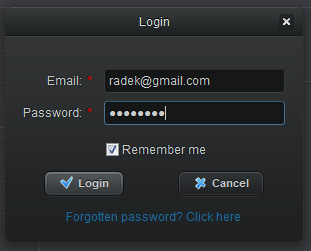
\includegraphics[width=0.5\textwidth]{./img/interfejsy/login2}
\caption{Okno logowania}
\label{fig:login}
\end{figure}

\subsection{Strona startowa}
\label{sec:start_page}

Po zalogowaniu na stronie startowej pojawiają się informacje o nadchodzących sesjach. Na rysunku \ref{fig:start_page_joined} ciemniejszym kolorem oznaczone są sesje, do których użytkownik w pełni dołączył, jaśniejszym --- oczekujące na akceptację przez założyciela ogłoszenia. Dla zalogowanych użytkowników możliwa jest nawigacja do kolejnych podstron --- zakładek.
\begin{figure}[htb]	
\centering
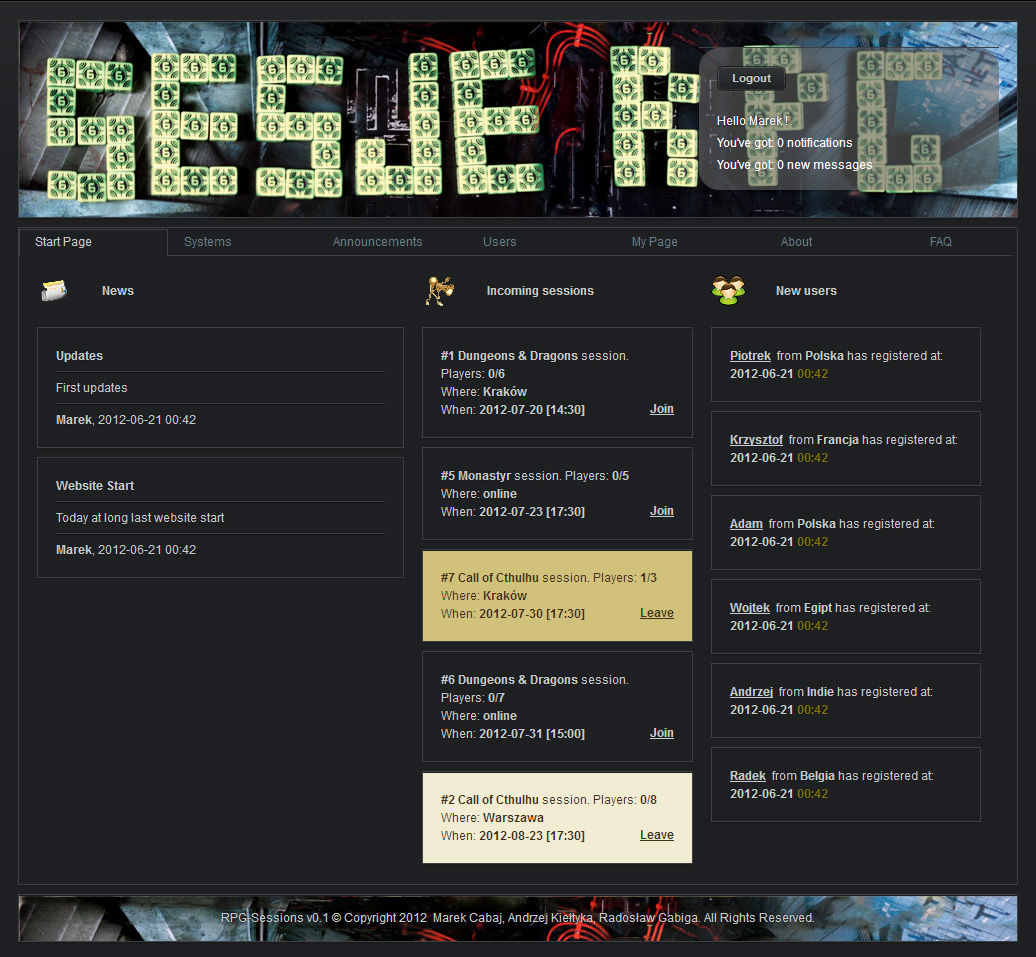
\includegraphics[width=0.9\textwidth]{./img/interfejsy/start_page_joined}
\caption{Strona startowa zalogowanego użytkownika}
\label{fig:start_page_joined}
\end{figure}

\subsection{Lista systemów}
\label{sec:systems}
Wybranie zakładki \emph{Systems} powoduje przejście do listy systemów RPG zapisanych w bazie serwisu. Składa się ona z tabeli systemów z podziałem na gatunki i rok wydania oraz opisu wybranej pozycji znajdującego się poniżej. Listę można filtrować względem pierwszej litery nazwy lub wyświetlać wszystko. Jeśli zalogowany użytkownik jest administratorem lub moderatorem, widoczne stają się przyciski \emph{New system}, \emph{Edit} i \emph{Delete} służące kolejno do dodawania nowego systemu, edycji istniejącego oraz usuwania. Całość przedstawia rysunek \ref{fig:systems}.

\begin{figure}[htb]	
\centering
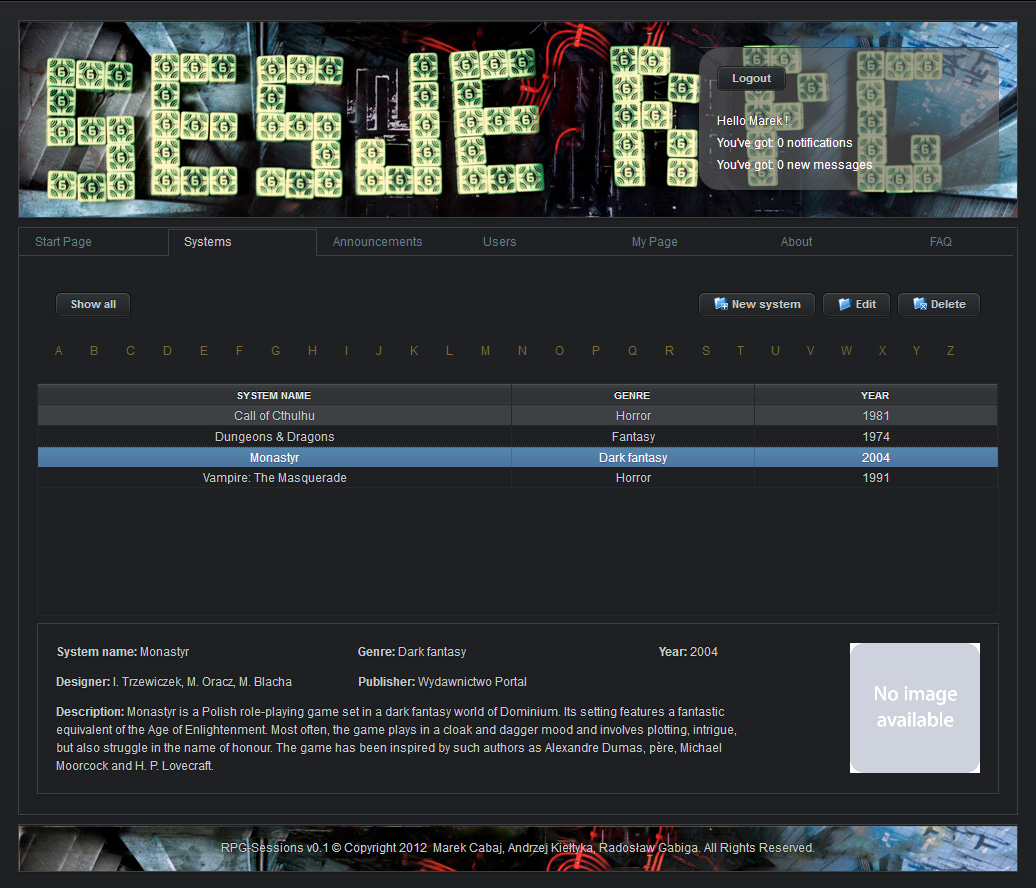
\includegraphics[width=0.9\textwidth]{./img/interfejsy/systems}
\caption{Lista systemów RPG}
\label{fig:systems}
\end{figure}

\subsection{Ogłoszenia}
\label{sec:sessions}
Zakładka \emph{Announcements} stanowi główny cel serwisu --- ogłoszenia o odbywających się sesjach (rys. \ref{fig:sessions}).  Znajduje się tutaj tabela z kluczowymi informacjami oraz rozwinięcie dostępne po zaznaczeniu wybranej pozycji. Sesje oznaczane są takimi samymi kolorami jak na stronie startowej. Po wybraniu sesji i naciśnięciu przycisku \emph{Join} pojawia się okno wyboru pozycji w~trakcie sesji (rys. \ref{fig:join_session}). Można dołączyć jako Mistrz Gry (\emph{Master}) lub jako Gracz (\emph{Player}). W~przypadku gdy dołączający użytkownik nie jest założycielem ogłoszenia, po wyborze pozycji wysyłana jest wiadomość z prośbą o akceptację do osoby odpowiedzialnej za sesję. 

\begin{figure}[htb]	
\centering
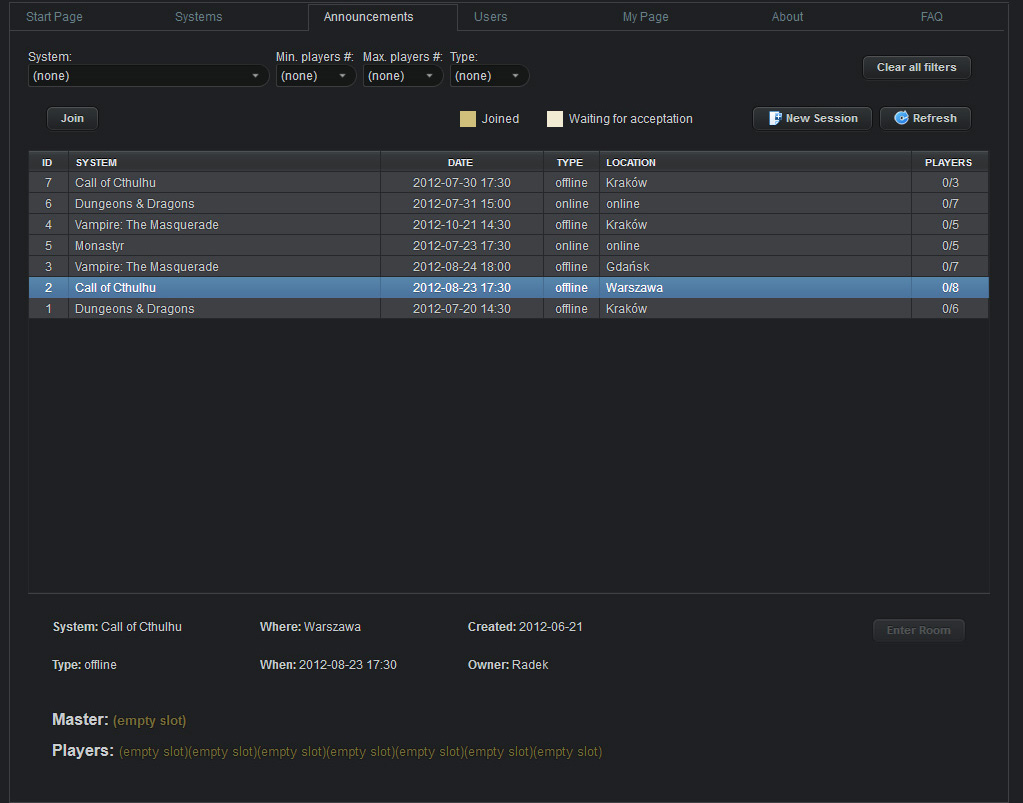
\includegraphics[width=0.9\textwidth]{./img/interfejsy/sessions}
\caption{Lista ogłoszeń}
\label{fig:sessions}
\end{figure}

\begin{figure}[htb]	
\centering
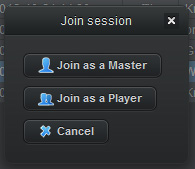
\includegraphics[width=0.3\textwidth]{./img/interfejsy/join_session}
\caption{Dołączanie do sesji}
\label{fig:join_session}
\end{figure}

Po naciśnięciu przycisku \emph{New Session} pojawia się okno tworzenia nowej sesji. Użytkownik podaje wymagane dane, wybiera czy od razu chce do niej dołączyć jako Gracz lub Mistrz Gry i dodaje ogłoszenie do bazy. Formularz ten jest przedstawiony na rysunku \ref{fig:create_session}.

\begin{figure}[htb]	
\centering
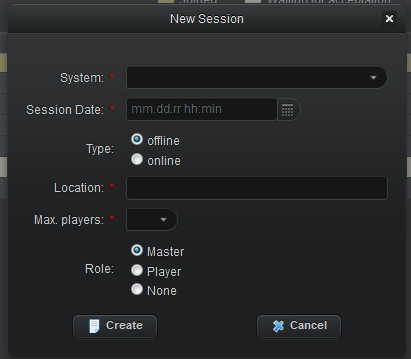
\includegraphics[width=0.7\textwidth]{./img/interfejsy/create_session}
\caption{Tworzenie nowej sesji}
\label{fig:create_session}
\end{figure}


%waiting for accepation ???


\subsection{Lista użytkowników}
\label{sec:users_detail}
Zakładka \emph{Users} (rys. \ref{fig:users_details} to lista użytkowników zamierająca pseudonim, datę dołączenia, kraj pochodzenia oraz status konta (aktywne, nieaktywne). Użytkownicy mogą wyświetlić szczegóły profilu po wybraniu danej osoby i naciśnięciu \emph{Show details}. Gdy zalogowany jest administrator lub moderator, widoczny jest również przycisk \emph{Deactivate account} służący do banowania użytkowników. 

\begin{figure}[htb]	
\centering
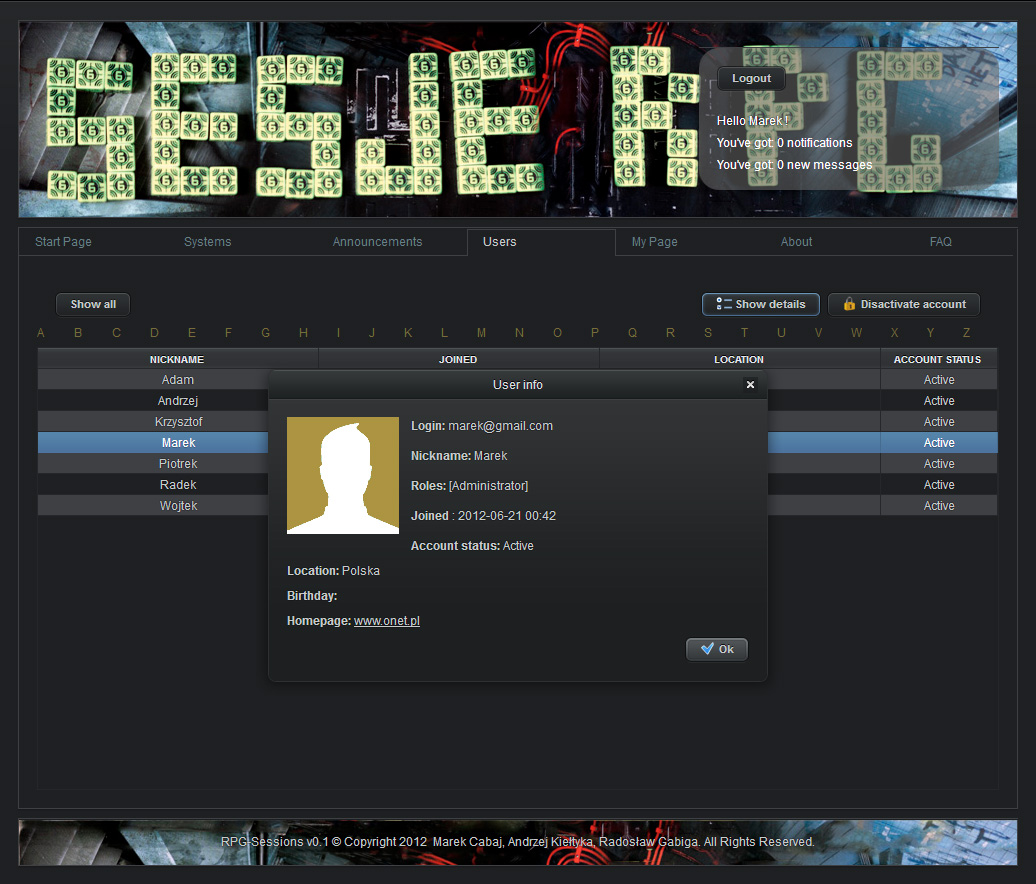
\includegraphics[width=0.9\textwidth]{./img/interfejsy/users_details}
\caption{Szczegóły profilu użytkownika}
\label{fig:users_details}
\end{figure}

\subsection{Strona profilowa}
\label{sec:my_page}
Zakładka \emph{My Page} zawiera profil zalogowanego użytkownika. Może tutaj przeglądać i edytować dane profilowe, sprawdzać wiadomości i powiadomienia systemowe, przeglądać sesje, w których uczestniczy, oczekuje na akceptacje lub które stworzył. Ponadto można tworzyć scenariusze rozgrywek jak i (w przyszłości) karty postaci. Administrator dodatkowo posiada możliwość dodawania wiadomości na stronę główną (\emph{News}) i pytań w dziale \emph{FAQ}. Przykład profilu ze stworzonymi sesjami przedstawia rysunek \ref{fig:mypage_sessions}.

\begin{figure}[htb]	
\centering
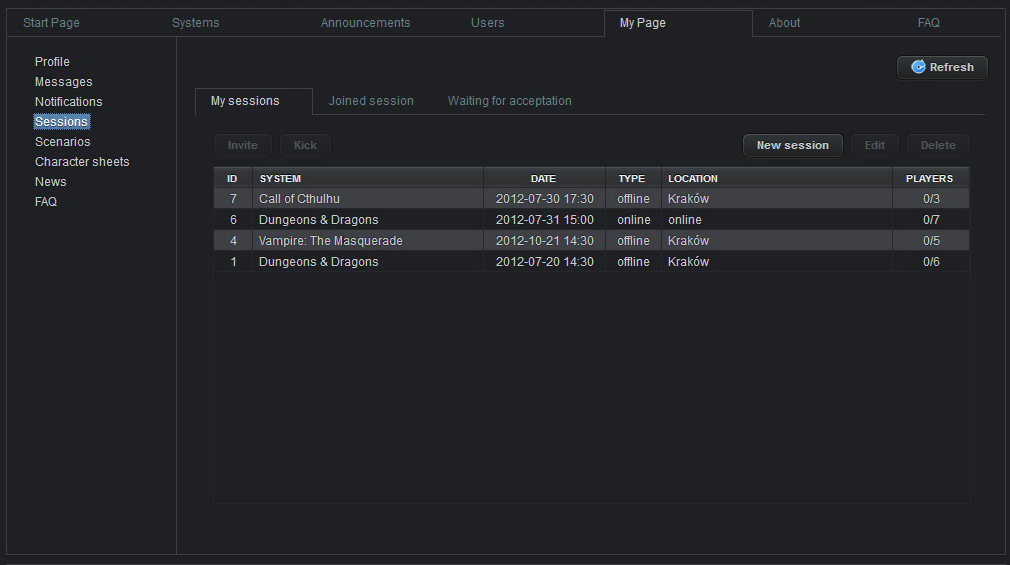
\includegraphics[width=0.9\textwidth]{./img/interfejsy/mypage_sessions}
\caption{Sesje użytkownika}
\label{fig:mypage_sessions}
\end{figure}

\subsection{FAQ}
\label{sec:faq}

\subsection{Edytowanie}
\label{sec:edit}

\subsection{Chat}
\label{sec:chat}

%obrazek chatu zrobić

%%%%%%%%%%%%%%%%%%%%%%%%%%%%%%%%%%%%%%%%

\section{Różnice pomiędzy projektem oraz implementacją}
\label{sec:roznice}

% TODO wszelkie różnice, zmiany

%%%%%%%%%%%%%%%%%%%%%%%%%%%%%%%%%%%%%%%%

\section{Rozwijanie i modyfikowanie aplikacji}
\label{sec:rozwoj}

% TODO co można oddać, rozwinąć, zmienić

%%%%%%%%%%%%%%%%%%%%%%%%%%%%%%%%%%%%%%%%

\section{Wnioski}
\label{sec:doswiadczenia}

% TODO wnioski